% !TEX root = main.tex
\section{Systemüberblick}
\label{sec:system}
In diesem Abschnitt wird die Systemstruktur gezeigt, sowie alle, zur Build- und Runtime relevanten, Komponenten von GraalVM Native Image erläutert.
Die Eingabe ist Java Bytecode, dieser kann dementsprechend von jeder JVM Sprache stammen, da diese zu Java Bytecode kompiliert werden. Der Anwendungscode, die benötigten Bibliotheken, das JDK und Teile einer virtuellen Maschine (SubstrateVM)\footnote{Umfasst u.A. Speicherverwaltung, Thread-Scheduling und Garbage Collection} werden zu Maschinencode kompiliert. Die resultierende, auf ein spezifisches Betriebssystem und Prozessorarchitektur angepasste, nativ ausführbare Datei(engl. executable) wird \textit{native image} genannt. Abbildung 1 zeigt die Komponenten und den Ablauf des Build-Vorgangs eines native image.

\begin{figure}[h]
	\centering
	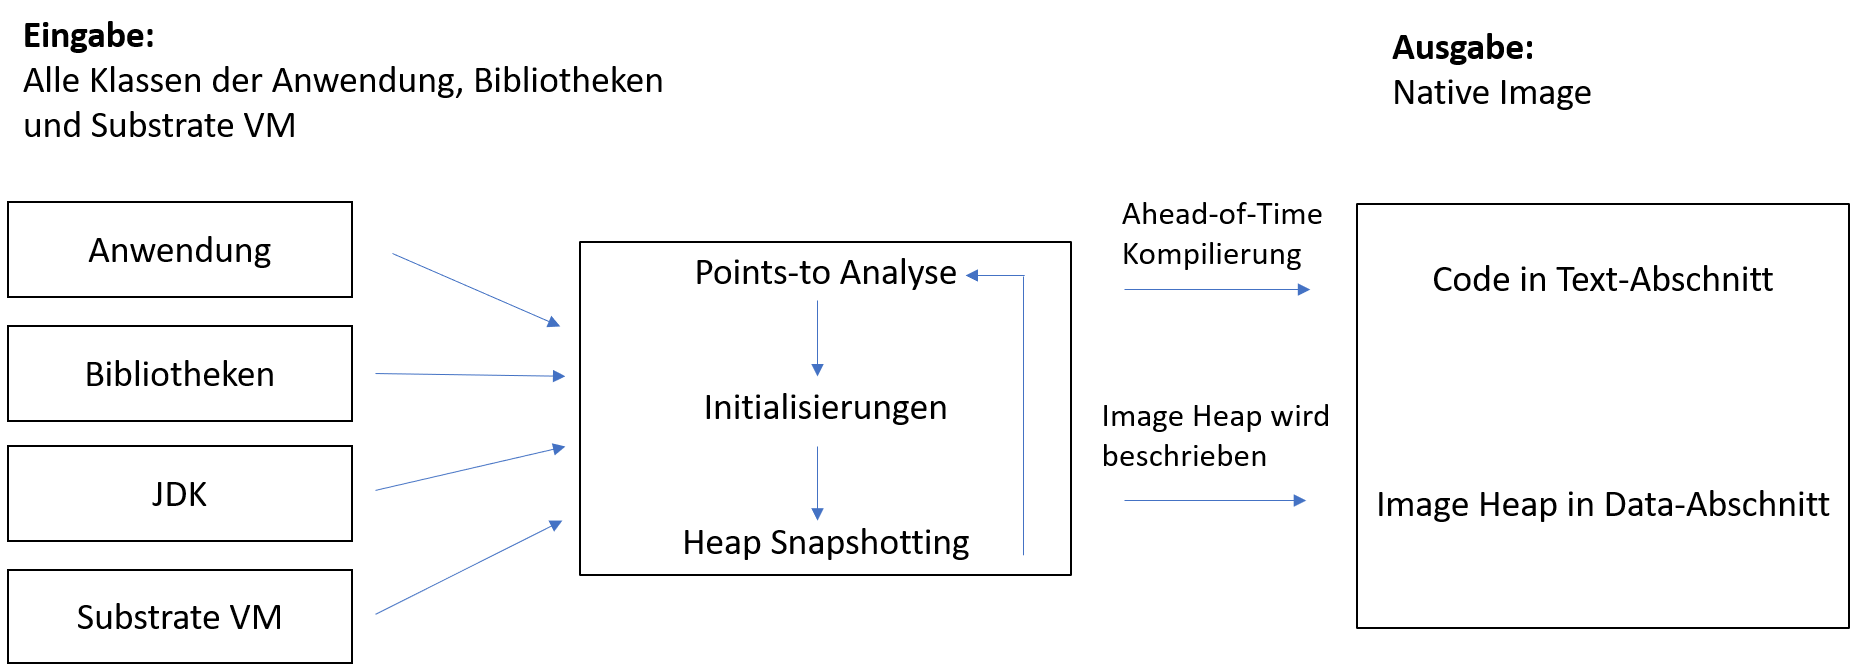
\includegraphics[width=1\textwidth]{resources/GraalVM_BuildTime.png}
	\caption{NativeImage Build-Vorgang}
	\label{fig:system_buildtime}
\end{figure}

\begin{todo}
	Bild überarbeiten, und neu einfügen.
\end{todo}

Die Points-To Analyse und das Heapsnapshotting werden iterativ durchgeführt bis ein definierter Punkt erreicht ist. Zudem werden die registrierten Callbacks der Anwendung, 
die über die Feature-API von GraalVM nutzbar sind, in diesem Zuge auch ausgeführt. Das Ergebnis dieses Prozesses ist eine Liste von, zur Laufzeit, erreichbaren Klassen, 
Methoden und Feldern, sowie ein Objekt-Graph mit erreichbaren Objekten. Im Letzten Schritt des Build-Vorgangs werden die erreichbaren Methoden zu Maschinencode kompiliert
 und der Objekt-Graph wird als \textit{image heap} ausgeschrieben, und in die Form des zur Laufzeit tatsächlich vorhandenen Heaps transformiert. Danach wird der Maschinencode 
 in die Text-Section, und der image heap in die Data-Section \cite[Fig. 1-13]{TISC1995} des native image geschrieben. Der gesamte Prozess wird \textit{image build time} genannt\cite{Wimmer2019}.
Die Anwendung welche die genannten Vorgänge übernimmt, ist der \textit{image builder}. Der \textit{image builder} selber ist eine Java-Anwendung. Sowohl die Pointer-Analyse 
und das ahead-of-time-Compiling, als auch das Ausführen der Klasseninitializer und Callback-Funktionen, werden also von ein und derselben Java VM
 übernommen\footnote{Das heißt wiederrum, dass bei der \textit{image build time}, die Objekte, aus denen sich der image heap zusammensetzt,
 normale Objekte im Java Heap des \textit{image builder} sind.
